\documentclass[7pt]{article}
\usepackage{amsmath}
\usepackage{graphicx}
\usepackage{caption}
\usepackage[landscape]{geometry}
\usepackage{multicol}
\usepackage{amssymb}
\usepackage{geometry}
 \geometry{
 a4paper,
 total={285mm,185mm},
 left=10mm,
 top=10mm,
 }
\setcounter{section}{0}
\setlength\columnseprule{0.5pt}
\setlength{\parindent}{0pt}
\graphicspath{ {images/} }

\begin{document}
\begin{multicols}{3}

\section{Allgemeines}


\subsection{SI Einheiten}

\begin{center}
	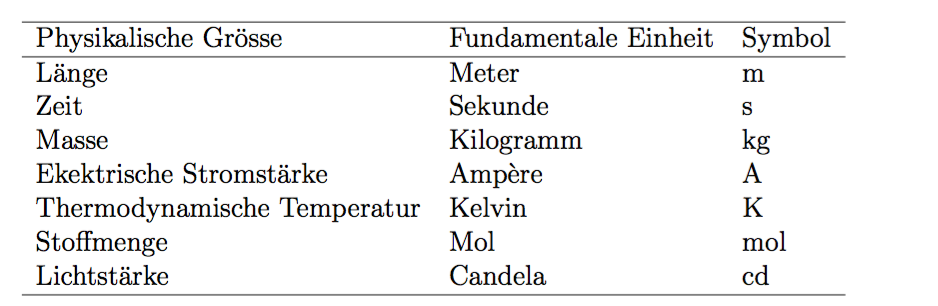
\includegraphics[width=250pt]{images/si_einheiten}
\end{center}



\subsection{Winkel}

\begin{equation}
	2\pi rad = 360°
\end{equation}
\begin{equation}
	1 \space rad = \frac{180}{\pi} \approx 57.296°
\end{equation}
\textbf {Umrechnen:}
\newline Radiant $\rightarrow$ Grad: Winkel*180°/$\pi$ 
\newline Grad $\rightarrow$ Radiant: Winkel*$\pi$/180°



\subsection{Raum und Zeit}

\textbf{Raum} = Abstand zwischen 2 Orten
\newline \textbf{Zeit} = Dauer bestimmter, reproduzierbarer Prozesse
\paragraph{Beispielgr{\"o}ssen}
\mbox{}\\ 
\begin{equation}
	1  \text{ pc} = 3,0857*10^{16} m = 206'247 \text{ A.U.}
\end{equation} 
wobei pc = Parsec und A.U. = Astronomical Unit = mittlerer Abstand zwischen Erde und Sonne
\newline
\newline Gr{\"o}sse des sichtbaren Universums $\approx 10^{10}$ pc 	
\newline Gr{\"o}sse der Milchstrasse (unsere Galaxie) $\approx 10^4$ pc
\newline Kleinste bekannte Gr{\"o}sse = Planksche L{\"a}nge $\approx 10^{-35}$ m
\newline
\newline Alter des Universums ca 4.3 * $10^{17}$ s
\newline Alter der Erde ca. 5 Milliarden Jahre
\newline Umlauf der Erde um die Sonne = 1 Jahr



\subsection{Koordinatensysteme}

Weil kein "absoluter" Punkt im Raum existiert, muss ein Punkt \textbf{P} im Raum immer bezüglich einem anderen Punkt \textbf{O (Ursprung)} definiert werden


\paragraph{Die kartesischen Koordinaten}

\mbox{}\\ Im kartesischen Koordinatensystem definiert man 3 zueinander senkrechte Richtungen x (vorne-hinten), y (links-rechts), z (oben-unten). Der Punkt P wird bezügl. des Ursprungs mit drei kartesischen Koordinaten lokalisiert:
\begin{equation}
	\textbf{OP} = (x,y,z) = (OA, OB, OC)
\end{equation}
wobei A = Projektion von P auf die x-Achse
\newline B = Projektion von P auf die y-Achse
\newline C = Projektion von P auf die z-Achse


\paragraph{Die Kugelkoordinaten}

\mbox{}\\
Im Kugelkoordinatensystem wird ein Punkt \textbf{P} im Raum durch 3 Koordinaten dargestellt, wobei 
\newline \textit{r} = Abstand zwischen \textbf{O} und \textbf{O}: \textbf{OP} = (r, $\vartheta, \varphi$) 
\newline $\vartheta$ = Winkel zwischen \textbf{OP} und z-Achse; 0 $\leq \vartheta \leq \pi$
\newline $\varphi$ = Winkel zwischen \textbf{OP'} und x-Achse; 0 $\leq \varphi \leq$ 2$\pi$
\begin{center}
	\includegraphics[width=200pt]{images/übergang_koordinatensysteme}
\end{center}
Wenn $\vartheta$ = $\frac{\pi}{2}$, dann liegt P auf der x-y-Ebene, man wird dann die zweidimensionalen \textbf{Polarkoordinaten} (r, $\varphi$) verwenden.


\paragraph{Umrechnen von Koordinatensystemen}

\mbox{}\\von Kugel- zu kartesischen Koordinaten:
\newline 
$\begin{pmatrix} 
	x \\ y \\ z 
\end{pmatrix} $ 
\textbf{=}
$\begin{pmatrix}
	r*sin\vartheta*cos\varphi \\ r*sin\vartheta*sin\varphi \\ r*cos\vartheta
\end{pmatrix}$
\newline
\newline
\newline von kartesischen zu Kugelkoordinaten:
\newline $\begin{pmatrix} 
	r \\ \varphi \\ \vartheta 
\end{pmatrix} $ 
\textbf{=}
$\begin{pmatrix}
	\sqrt{x^{2}+ y^{2} + z^{2}} \\ arctan(\frac{y}{x}) \\ arccos(\frac{z}{r})
\end{pmatrix}$

\paragraph{Zylinderkoordinaten}

\mbox{}\\ Zylindrische Koordinaten sind Polarkoordinaten mit einer dritten, senkrechten, Koordinaten ergänzt. 
\begin{equation}
	\textbf{OP} = (\rho, \varphi, z)
\end{equation}

von Zylinder- zu kartesischen Koordinaten:
\newline 
$\begin{pmatrix} 
	x \\ y \\ z 
\end{pmatrix} $ 
\textbf{=}
$\begin{pmatrix}
	\rho*cos\varphi \\ \rho*sin\varphi \\ z
\end{pmatrix}$
\newline
\newline
\newline von kartesischen zu Zylinderkoordinaten:
\newline $\begin{pmatrix} 
	\rho \\ \varphi \\ z 
\end{pmatrix} $ 
\textbf{=}
$\begin{pmatrix}
	\sqrt{x^{2}+ y^{2}} \\ arctan(\frac{y}{x}) \\ z
\end{pmatrix}$



\subsection{Vektoren}

\mbox{}
\textbf{Skalarprodukt:} \begin{equation}
	a \cdot b = |a||b| cos\varphi
\end{equation}
\begin{equation}
	a \cdot b = a_{x} b_{x} + a_{y} b_{y} + a_{z} b_{z}	
\end{equation}

wobei  $\varphi$ der Winkel zwischen den beiden Vektoren a und b ist. Wenn das Skalarprodukt verschwindet, ist a oder b = 0 oder die beiden Vektoren stehen senkrecht aufeinander.
\newline
\newline \textbf{Cosinussatz:}
\begin{equation}
	|c^|{2} = |a|^{2} + |b|^{2} + 2|a||b|cos\varphi
\end{equation}
\textbf{Vektorprodukt:}
\begin{equation}
	c = a \times b = -b \times a
\end{equation}
\begin{equation}
	a \times b = (a_{y}b_{z} - a_{z}b_{y})e_{x} +  (a_{z}b_{x} - a_{x}b_{z})e_{y}	 +  (a_{x}b_{y} - a_{y}b_{x})e_{z}	
\end{equation}
\begin{equation}
	c = ab sin \varphi
\end{equation}
wobei der Betrag des Vektors \textbf{c} gleich der Fläche des Parallelogramms ist, welche \textbf{a} und \textbf{b} aufspannen. \textbf{c} steht senkrecht auf \textbf{a} und \textbf{b}. Wenn die Vektoren parallel sind, ist das Vektorprodukt gleich 0. 


\
	
\end{multicols}
\end{document}